% SPDX-FileCopyrightText: 2026 Onur Tuncer and Stereon contributors
% SPDX-License-Identifier: MPL-2.0
%
% This Source Code Form is subject to the terms of the Mozilla Public
% License, v. 2.0. If a copy of the MPL was not distributed with this
% file, You can obtain one at https://mozilla.org/MPL/2.0/.
%
% A solid as its boundary (docs/intro.rst): the topology of a box (a face,
% the loop of coedges that bounds it, an edge, a vertex) and the geometry
% each entity is attached to (a plane, a line, a point). The topology says
% how the pieces connect; the geometry says where they are.
\documentclass[tikz,border=6pt]{standalone}
\usetikzlibrary{calc,arrows.meta,decorations.markings}
\definecolor{face}{RGB}{31,119,180}
\definecolor{edge}{RGB}{214,39,40}
\definecolor{vert}{RGB}{44,160,44}
\definecolor{geom}{RGB}{90,90,90}
\begin{document}
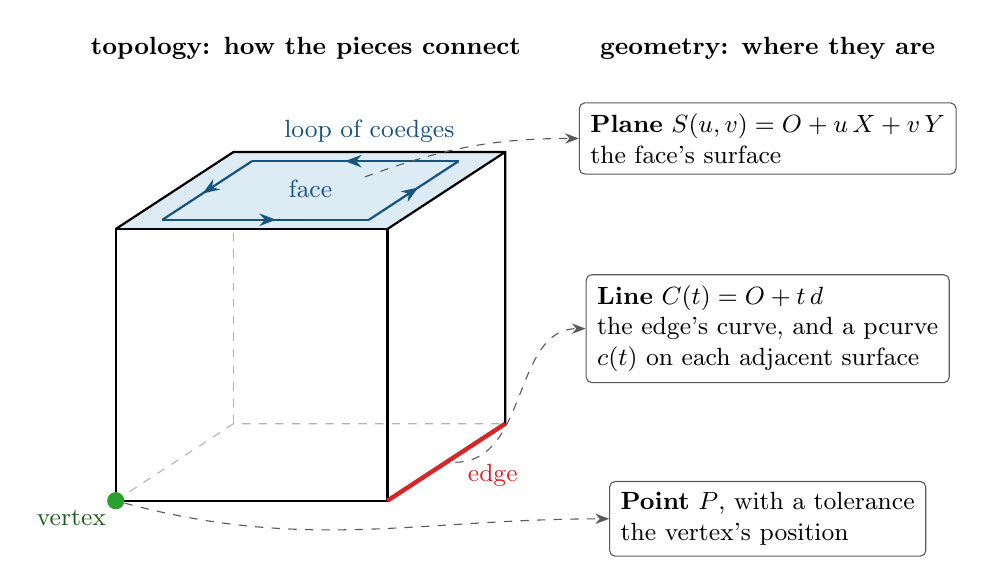
\begin{tikzpicture}[scale=1.15,
    lbl/.style={font=\small},
    geo/.style={font=\small,draw=geom,rounded corners=2pt,fill=white,inner sep=4pt,align=left},
    link/.style={geom,dashed,-{Stealth[length=5pt]}},
    coedge/.style={face!70!black,thick,
      postaction={decorate},
      decoration={markings,mark=at position 0.55 with {\arrow{Stealth[length=6pt]}}}}]
  % A box in oblique projection: front square and the back one behind it.
  \coordinate (off) at (1.3,0.85);
  \coordinate (A) at (0,0);   \coordinate (B) at (3,0);
  \coordinate (C) at (3,3);   \coordinate (D) at (0,3);
  \coordinate (A') at ($(A)+(off)$); \coordinate (B') at ($(B)+(off)$);
  \coordinate (C') at ($(C)+(off)$); \coordinate (D') at ($(D)+(off)$);

  % Hidden edges
  \draw[gray!60,dashed] (A) -- (A') -- (B');
  \draw[gray!60,dashed] (A') -- (D');
  % The top face, shaded
  \fill[face!15] (D) -- (C) -- (C') -- (D') -- cycle;
  % Visible edges
  \draw[thick] (A) -- (B) -- (C) -- (D) -- cycle;
  \draw[thick] (B) -- (B') -- (C') -- (D') -- (D);
  \draw[thick] (C) -- (C');
  % One edge, highlighted
  \draw[edge,ultra thick] (B) -- (B');
  % The top face's loop of coedges, inset from its boundary, counter-clockwise
  % about its outward normal
  \begin{scope}
    \coordinate (d) at ($(D)!0.12!(C')$);   \coordinate (c) at ($(C)!0.12!(D')$);
    \coordinate (c') at ($(C')!0.12!(D)$);  \coordinate (d') at ($(D')!0.12!(C)$);
    \draw[coedge] (d) -- (c);
    \draw[coedge] (c) -- (c');
    \draw[coedge] (c') -- (d');
    \draw[coedge] (d') -- (d);
  \end{scope}
  % One vertex
  \node[circle,fill=vert,inner sep=2.2pt] (V) at (A) {};

  % Labels on the topology
  \node[lbl,face!70!black] at ($(D)!0.5!(C')+(0,0.02)$) {face};
  \node[lbl,face!70!black,above] at ($(D')!0.5!(C')$) {loop of coedges};
  \node[lbl,edge,below right] at ($(B)!0.6!(B')$) {edge};
  \node[lbl,vert!60!black,below left] at (A) {vertex};

  % The geometry each entity carries
  \node[geo] (Gs) at (7.2,4.0) {\textbf{Plane} $S(u,v) = O + u\,X + v\,Y$\\
                                    the face's surface};
  \node[geo] (Gc) at (7.2,1.9) {\textbf{Line} $C(t) = O + t\,d$\\
                                    the edge's curve, and a pcurve\\
                                    $c(t)$ on each adjacent surface};
  \node[geo] (Gp) at (7.2,-0.2) {\textbf{Point} $P$, with a tolerance\\
                                    the vertex's position};
  \draw[link] ($(D)!0.5!(C')+(0.6,0.15)$) to[out=20,in=180] (Gs.west);
  \draw[link] ($(B)!0.5!(B')+(0.1,0)$) to[out=0,in=180] (Gc.west);
  \draw[link] (V) to[out=-15,in=180] (Gp.west);

  % Headings
  \node[font=\small\bfseries] at (2.1,5.0) {topology: how the pieces connect};
  \node[font=\small\bfseries] at (7.2,5.0) {geometry: where they are};
\end{tikzpicture}
\end{document}
